\chapter{Consistency and Consensus}
\emph{Anm.: Quelle ist hier der deutsche Tanenbaum/Steen, daher sind manche englischen Begriffe evtl. nicht korrekt gewählt.}

\paragraph{}
\begin{compactitem}
	\item Distributed Systems use replication of data to improve \emph{performance} and/or \emph{reliability}
	\item replication for scalability\\
	How to keep replicas consistent?\\
	Many types of consistency\\
	\begin{compactitem}
		\item data-centric-constistency
		\item client-centric-consistency
	\item monotic reads: successive reads return the same or newer value
	\item monitic write: a write op must be completed before the next write by the same process
	\item read-your-own-write: write is always seen by read of same process
	\item write-follows-read: write on previous read takes place on the same or more recent value
	\end{compactitem}
	\item Do not discuss replica placement
        \item Object-replication
        % evtl TODO
\end{compactitem}
\section{Data-centric consistency}
The more strict a model is, the stronger are the assumptions, that may be drawn from a series of events, but the harder to implement.

\subsection{Strict consistency}
\emph{Every read of x returns the value of the last write on x}
\paragraph{Example strict consistency}
\begin{tabbing}
P1: W(x)a \= \\
\rule{0.3\textwidth}{0.4pt} \\
P2: \> R(x)a
\end{tabbing}
\paragraph{Non strict consistent example}
\begin{tabbing}
P1: W(x)a \= \\
\rule{0.3\textwidth}{0.4pt} \\
P2: \> R(x)Null \ R(x)a
\end{tabbing}

\paragraph{}
Simple and clear idea, but this definition requires existence of global time (hard to realise), so that the \emph{last} write on a variable is unambiguous. This requirement is very hard to accomplish.

If a data storage fulfills this requirement, then every write must be visible globally (for every process in the system).

\subsection{Sequential/linear consistency}
Weak version of strict consistency, irrelevance of the chronological order of write events.
That means, that there is no global time or chronology, but some order of the events is globally visible and the same for every process.
Linear consistency just adds the requirement, that the events are ordered by a globally (mayhaps ambiguous) timestamp.
\paragraph{Example sequential consistency}
\begin{tabbing}
P1: W(x)a \= \\
\rule{0.4\textwidth}{0.4pt} \\
P2: \> W(x)b \= \\
\rule{0.4\textwidth}{0.4pt} \\
P3: \> \> R(x)b \= \hspace{32pt} \= R(x)a \\
\rule{0.4\textwidth}{0.4pt} \\
P4: \> \> \> \= R(x)b \hspace{5pt} \= R(x)a \\
\end{tabbing}

\paragraph{Example non-sequential consistency}
\begin{tabbing}
P1: W(x)a \= \\
\rule{0.4\textwidth}{0.4pt} \\
P2: \> W(x)b \= \\
\rule{0.4\textwidth}{0.4pt} \\
P3: \> \> R(x)b \= \hspace{32pt} \= R(x)a \\
\rule{0.4\textwidth}{0.4pt} \\
P4: \> \> \> \= R(x)a \hspace{5pt} \= R(x)b \\
\end{tabbing}

\subsection{Causal consistency}
Weak version of sequential consistency, only causally dependent events must appear strictly ordered on a global level.
Two causally dependent events may be a write event \emph{W(x)a}, a read event \emph{R(x)a} followed by a write \emph{W(x)b}, then the write \emph{W(x)b} may be based on the value writte in \emph{W(x)a}.
\paragraph{Example causal consistency}
\begin{tabbing}
P1: W(x)a \= \hspace{64pt} W(x)c \= \\
\rule{0.5\textwidth}{0.4pt} \\
P2: \> R(x)a \hspace{5pt} W(x)b \\
\rule{0.5\textwidth}{0.4pt} \\
P3: \> R(x)a \> R(x)c \hspace{5pt} R(x)b \\
\rule{0.5\textwidth}{0.4pt} \\
P4: \> R(x)a \> R(x)b \hspace{5pt} R(x)c \\
\end{tabbing}
\paragraph{Example non-causal consistency}
\begin{tabbing}
P1: W(x)a \= \\
\rule{0.4\textwidth}{0.4pt} \\
P2: \> R(x)a \hspace{5pt} W(x)b \= \\
\rule{0.4\textwidth}{0.4pt} \\
P3: \> \> R(x)b \hspace{5pt} R(x)a \\
\rule{0.4\textwidth}{0.4pt} \\
P4: \> \> R(x)a \hspace{5pt} R(x)b \\
\end{tabbing}

\subsection{FIFO-consistency}
Weak version of causal consitency.
The writes of a single process (which are ordered and causally dependent) appear in this exact order globally, but the sequence of writes between multiple processes is not strictly ordered. In other words, only the casual dependencies inside one process appear in the correct order, dependencies between different processes may be mixed.
\paragraph{Example FIFO-consistency}
\begin{tabbing}
P1: W(x)a \= \\
\rule{0.6\textwidth}{0.4pt} \\
P2: \> R(x)a \hspace{5pt} W(x)b \hspace{5pt} W(x)c \= \\
\rule{0.6\textwidth}{0.4pt} \\
P3: \> \> R(x)b \hspace{5pt} \= R(x)a \hspace{5pt} \= R(x)c \\
\rule{0.6\textwidth}{0.4pt} \\
P4: \> \> R(x)a \> R(x)b \> R(x)c \\
\end{tabbing}

\subsection{Weak consistency}
The idea of weak consistency is, that also the relatively weak assertions of FIFO-consistency often are too hard to implement or just unnecessary. The globally visible actions are reduced to critical sections (or areas) where the actions become globally visible only after leaving the critical section, so only the results of the actions become visible.
To realise that behaviour a mechanism to synchronise on the current state of a synchronisation variable \( S \) is introduced, such that processes who are interested in the current status of this variable may update their data, but other processes are not bothered with updates.

In this consistency scheme, consistency is not defined absolutely but only temporarily (at synchronization points).
\paragraph{Example weak consistency}
\begin{tabbing}
P1: W(x)a \hspace{5pt} W(x)b \hspace{5pt} S \hspace{5pt} \= \\
\rule{0.5\textwidth}{0.4pt} \\
P2: \> R(x)a \hspace{5pt} \= R(x)b \hspace{5pt} S \\
\rule{0.5\textwidth}{0.4pt} \\
P3: \> R(x)b \hspace{5pt} \= R(x)a \hspace{5pt} S \\
\end{tabbing}

\paragraph{Example non-weak consistency}
\begin{tabbing}
P1: W(x)a \hspace{5pt} W(x)b \hspace{5pt} S \hspace{5pt} \= \\
\rule{0.4\textwidth}{0.4pt} \\
P2: \> S \hspace{5pt} R(x)a \hspace{5pt} \\
\end{tabbing}

\subsection{Release-consistency}
In the weak-consistency-scheme there is no difference between synchronising after a write (i.e. a write-through to all replications) and synchronising before reading data, but these two scenarios require different actions on lower layers.
Two additional procedures are added \emph{acquire(..)} and \emph{release(..)}.

\subsection{Entry-consistency}
Similar to release-consistency, but synchronisation variables (and procedures acq(..), rel(..)) are responsible for a designated set of variables, not for all variables in the global scope.

\section{Client-centric consistency}
In contrast to the data-centric consistency models client-centric consistency models do not try to maintain a system wide consistent view, but rather try to hide inconsitencies on client level.

\subsection{Eventual consistency}
(popular example: Domain Name Service)
Usually big, distributed, replicated databases, which tolerate a high amount of incostency, but eventually become consistent when there are no updates to the database.
It is important that clients access the system via fixed nodes, otherwise client updates may take a while, until they are visible for the client itself which is a clear violation of local consistency (read your writes).
Remember that in this section the consistency view is only local/client-specific!

\subsection{Monotone read-consistency}
\emph{When a datum x is read by a process, then every following read of x results in the same value, or in newer value.}

\subsection{Monotone write-consistency}
\emph{When a process writes to a datum x, then all previous write operations have to be finished/applied.}

\subsection{Read your writes}
\emph{The result of a previous write operation of a process on a datum x is always visible in a following read of the same process}

\subsection{Writes follow reads}
\emph{A write by a process to a datum x, which follows a previous read of x, is performed on this read value, or a newer one.}

\subsection{Implementing client-side consistency}
The idea here is to monitor the client's reads and writes and add an ID to each operation. When reading/writing to a server the current status of the client (a list of the reads/writes) is added to the query and the server checks, wether the local storage of the client has to be updatet before executing the query.

\section{Reliable multicast protocols}
\begin{compactitem}
	\item atomic multicast requirement\\
	all requests arrive at all servers in the same order
\end{compactitem}
\subsection{Distributed Commit}
\begin{compactitem}
	\item an operatio is performed by group or non of the nodes of the group
	\item reliable multicast operation = delivery of message
	\item distributed transaction: operation = execution of transaction
	\item uses coordinator
	\item one-phased commit
	%bild?
	\begin{compactitem}
	\item distributed transaction involves several processors each on a different machine\\
	2 phases with each 2 steps:\\
	\begin{compactenum}
		\item coordinator $\xrightarrow{vote\ request}$ all participants
		\item participant $\xrightarrow[vote\ abort]{vote\ commit}$ coordinator
		\item if all commit\\
		coordinator $\xrightarrow{global-commit}$ all participants\\
		else\\
		coordinator $\xrightarrow{global-abort}$ all participants\\
		\item if commit, then participants locally commit\\
		else participants locally abort\\
			\begin{minipage}{\linewidth}
			\centering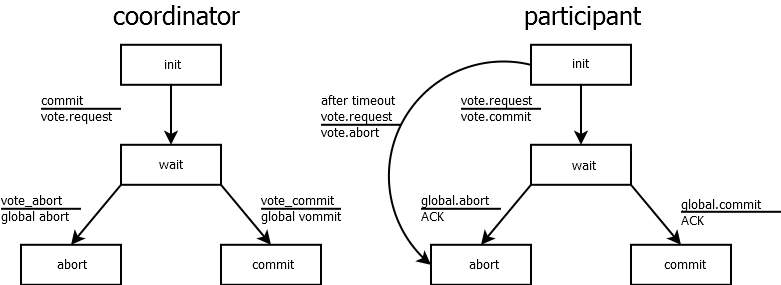
\includegraphics[width=310px]{gfx/2pc.png}
			\captionof{figure}{2PC}
			\label{img:2pc}
			\end{minipage}
		\item two-phase commit (2PC) (Jim Gray, 1978)
	\end{compactenum}
	Problems if failures occur\\
	\begin{compactitem}
		\item coordinator blocks in: wait
		\item participant blocks in: ready, init
	\end{compactitem}
	$\Rightarrow$ blocking commit protocol
	\item use timeouts to unblock
	\item repeat request
	\item in state ready P con contact Q\\
	if Q is in contact, then coordinator died after sending to Q\\
	before sending to P $\Rightarrow$ P can commit\\
	if Q is in abort $\Rightarrow$ abort\\
	if Q is in init $\Rightarrow$ abort\\
	if Q is in ready $\rightarrow$ abort or no decision contact R\\
	\end{compactitem}
	\item Three-phase commit (3PC) (Steen, 1981)\\
	\begin{compactitem}
		\item avoids blocking in the presence of fail-stop crashes
		\item states satisfy the following conditions\\
		\begin{compactenum}
			\item there is no state from which directly follow commit or abort follows
			\item there is no state in which it is not possible to make a final decision and from which a transaction to a commit state can be made
		\end{compactenum}
		$\Rightarrow$ necessary and sufficient conditions for non-blocking commit protocol\\
			\begin{minipage}{\linewidth}
			\centering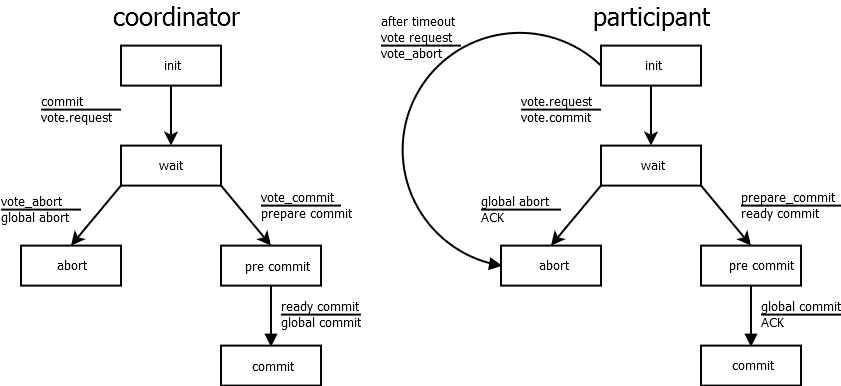
\includegraphics[width=310px]{gfx/3pc.png}
			\captionof{figure}{3PC}
			\label{img:3pc}
			\end{minipage}
		\item abort branch as in 2PC
		\item blocking states: paritcipant: init -> abort\\
		coordinator: wait --> abort\\
		precommit, knowing P voted for commit\\
		$\Rightarrow$ global-commit+recovery of P\\
		participant: ready\\
			coordinator failed as in 2PC\\
			precommit: contact other participants: if Q in precommit $\Rightarrow$ commit\\
			if Q is in init $\Rightarrow$ abort
		\item Q can be in INIT only if no participant is in precommit
		\item participant can reach precommit only if coordinator was in precommit already
		\item In 2PC a crashed participant could recover to commit, while all others are still in ready
		\item if one process is in ready recovery can be only to states ready, init, abort, precommit\\
		$\Rightarrow$ surviving processes can come to final solution
	\end{compactitem}
	\item Paxos (Leslie Lamport, late 80s)
	\begin{compactitem}
		\item does not block with at most n/2-1 failures\\
		%Bild!!!! <- Tobi!!!!
		Paxos adds to 2PC:
		\begin{compactitem}
			\item ordering of proposals
			\item majority voting for acceptance
		\end{compactitem}
		Duelling proposer
	\end{compactitem}
\end{compactitem}


